% Options for packages loaded elsewhere
\PassOptionsToPackage{unicode}{hyperref}
\PassOptionsToPackage{hyphens}{url}
%
\documentclass[
]{article}
\usepackage{lmodern}
\usepackage{amssymb,amsmath}
\usepackage{ifxetex,ifluatex}
\ifnum 0\ifxetex 1\fi\ifluatex 1\fi=0 % if pdftex
  \usepackage[T1]{fontenc}
  \usepackage[utf8]{inputenc}
  \usepackage{textcomp} % provide euro and other symbols
\else % if luatex or xetex
  \usepackage{unicode-math}
  \defaultfontfeatures{Scale=MatchLowercase}
  \defaultfontfeatures[\rmfamily]{Ligatures=TeX,Scale=1}
\fi
% Use upquote if available, for straight quotes in verbatim environments
\IfFileExists{upquote.sty}{\usepackage{upquote}}{}
\IfFileExists{microtype.sty}{% use microtype if available
  \usepackage[]{microtype}
  \UseMicrotypeSet[protrusion]{basicmath} % disable protrusion for tt fonts
}{}
\makeatletter
\@ifundefined{KOMAClassName}{% if non-KOMA class
  \IfFileExists{parskip.sty}{%
    \usepackage{parskip}
  }{% else
    \setlength{\parindent}{0pt}
    \setlength{\parskip}{6pt plus 2pt minus 1pt}}
}{% if KOMA class
  \KOMAoptions{parskip=half}}
\makeatother
\usepackage{xcolor}
\IfFileExists{xurl.sty}{\usepackage{xurl}}{} % add URL line breaks if available
\IfFileExists{bookmark.sty}{\usepackage{bookmark}}{\usepackage{hyperref}}
\hypersetup{
  pdftitle={BIOS 7659 Homework 4},
  pdfauthor={Tim Vigers},
  hidelinks,
  pdfcreator={LaTeX via pandoc}}
\urlstyle{same} % disable monospaced font for URLs
\usepackage[margin=1in]{geometry}
\usepackage{color}
\usepackage{fancyvrb}
\newcommand{\VerbBar}{|}
\newcommand{\VERB}{\Verb[commandchars=\\\{\}]}
\DefineVerbatimEnvironment{Highlighting}{Verbatim}{commandchars=\\\{\}}
% Add ',fontsize=\small' for more characters per line
\usepackage{framed}
\definecolor{shadecolor}{RGB}{248,248,248}
\newenvironment{Shaded}{\begin{snugshade}}{\end{snugshade}}
\newcommand{\AlertTok}[1]{\textcolor[rgb]{0.94,0.16,0.16}{#1}}
\newcommand{\AnnotationTok}[1]{\textcolor[rgb]{0.56,0.35,0.01}{\textbf{\textit{#1}}}}
\newcommand{\AttributeTok}[1]{\textcolor[rgb]{0.77,0.63,0.00}{#1}}
\newcommand{\BaseNTok}[1]{\textcolor[rgb]{0.00,0.00,0.81}{#1}}
\newcommand{\BuiltInTok}[1]{#1}
\newcommand{\CharTok}[1]{\textcolor[rgb]{0.31,0.60,0.02}{#1}}
\newcommand{\CommentTok}[1]{\textcolor[rgb]{0.56,0.35,0.01}{\textit{#1}}}
\newcommand{\CommentVarTok}[1]{\textcolor[rgb]{0.56,0.35,0.01}{\textbf{\textit{#1}}}}
\newcommand{\ConstantTok}[1]{\textcolor[rgb]{0.00,0.00,0.00}{#1}}
\newcommand{\ControlFlowTok}[1]{\textcolor[rgb]{0.13,0.29,0.53}{\textbf{#1}}}
\newcommand{\DataTypeTok}[1]{\textcolor[rgb]{0.13,0.29,0.53}{#1}}
\newcommand{\DecValTok}[1]{\textcolor[rgb]{0.00,0.00,0.81}{#1}}
\newcommand{\DocumentationTok}[1]{\textcolor[rgb]{0.56,0.35,0.01}{\textbf{\textit{#1}}}}
\newcommand{\ErrorTok}[1]{\textcolor[rgb]{0.64,0.00,0.00}{\textbf{#1}}}
\newcommand{\ExtensionTok}[1]{#1}
\newcommand{\FloatTok}[1]{\textcolor[rgb]{0.00,0.00,0.81}{#1}}
\newcommand{\FunctionTok}[1]{\textcolor[rgb]{0.00,0.00,0.00}{#1}}
\newcommand{\ImportTok}[1]{#1}
\newcommand{\InformationTok}[1]{\textcolor[rgb]{0.56,0.35,0.01}{\textbf{\textit{#1}}}}
\newcommand{\KeywordTok}[1]{\textcolor[rgb]{0.13,0.29,0.53}{\textbf{#1}}}
\newcommand{\NormalTok}[1]{#1}
\newcommand{\OperatorTok}[1]{\textcolor[rgb]{0.81,0.36,0.00}{\textbf{#1}}}
\newcommand{\OtherTok}[1]{\textcolor[rgb]{0.56,0.35,0.01}{#1}}
\newcommand{\PreprocessorTok}[1]{\textcolor[rgb]{0.56,0.35,0.01}{\textit{#1}}}
\newcommand{\RegionMarkerTok}[1]{#1}
\newcommand{\SpecialCharTok}[1]{\textcolor[rgb]{0.00,0.00,0.00}{#1}}
\newcommand{\SpecialStringTok}[1]{\textcolor[rgb]{0.31,0.60,0.02}{#1}}
\newcommand{\StringTok}[1]{\textcolor[rgb]{0.31,0.60,0.02}{#1}}
\newcommand{\VariableTok}[1]{\textcolor[rgb]{0.00,0.00,0.00}{#1}}
\newcommand{\VerbatimStringTok}[1]{\textcolor[rgb]{0.31,0.60,0.02}{#1}}
\newcommand{\WarningTok}[1]{\textcolor[rgb]{0.56,0.35,0.01}{\textbf{\textit{#1}}}}
\usepackage{longtable,booktabs}
% Correct order of tables after \paragraph or \subparagraph
\usepackage{etoolbox}
\makeatletter
\patchcmd\longtable{\par}{\if@noskipsec\mbox{}\fi\par}{}{}
\makeatother
% Allow footnotes in longtable head/foot
\IfFileExists{footnotehyper.sty}{\usepackage{footnotehyper}}{\usepackage{footnote}}
\makesavenoteenv{longtable}
\usepackage{graphicx,grffile}
\makeatletter
\def\maxwidth{\ifdim\Gin@nat@width>\linewidth\linewidth\else\Gin@nat@width\fi}
\def\maxheight{\ifdim\Gin@nat@height>\textheight\textheight\else\Gin@nat@height\fi}
\makeatother
% Scale images if necessary, so that they will not overflow the page
% margins by default, and it is still possible to overwrite the defaults
% using explicit options in \includegraphics[width, height, ...]{}
\setkeys{Gin}{width=\maxwidth,height=\maxheight,keepaspectratio}
% Set default figure placement to htbp
\makeatletter
\def\fps@figure{htbp}
\makeatother
\setlength{\emergencystretch}{3em} % prevent overfull lines
\providecommand{\tightlist}{%
  \setlength{\itemsep}{0pt}\setlength{\parskip}{0pt}}
\setcounter{secnumdepth}{-\maxdimen} % remove section numbering

\title{BIOS 7659 Homework 4}
\author{Tim Vigers}
\date{20 October 2020}

\begin{document}
\maketitle

\hypertarget{rna-seq-data-and-qc}{%
\section{1. RNA-seq Data and QC}\label{rna-seq-data-and-qc}}

\hypertarget{a-read-information}{%
\subsection{a) Read information}\label{a-read-information}}

The first entry in the .fastq file is:

`@SRR390924.1.1 COLUMBO:1:1:1:1926 length=36

AAAAAAAANAAAAAAAAAAAAAAAAAAAAAAAAAAA

+SRR390924.1.1 COLUMBO:1:1:1:1926 length=36

\#\#\#\#\#\#\#\#\#\#\#\#\#\#\#\#\#\#\#\#\#\#\#\#\#\#\#\#\#\#\#\#\#\#\#\#`

The first line contains the sequence ID (after the @ symbol) and an
optional description. Line 2 contains the read sequence and line 3 has
the same sequence ID (this time after the + symbol) followed by another
optional description. The final line encodes a quality score for each
base pair (BP) in the sequence using the hexadecimal format. In this
dataset, reads are 36 BP long.

For more recent Illumina systems, you can find the q-score for each BP
by subtracting 33 from the ASCII code. From the q-score you can then
calculate the probability that the BP call was incorrect using the
formula \(P=10^{\frac{-Q}{10}}\). For for the first entry in this file,
\(q=35-33=2\), so \(P=\) 0.631. This is not a high quality read.

According to the SRA entry there are 3,614,610 reads in this file.

\hypertarget{b-summary-statistics}{%
\subsection{b) Summary statistics}\label{b-summary-statistics}}

``FASTQ Summary Statistics'' returns a table where each row represents a
BP position within a read (in this case 1-36). For each BP position, the
table includes quality summary statistics such as minimum, maximum, and
mean q-score. It also lists base counts and potential outliers:

\begin{Shaded}
\begin{Highlighting}[]
\NormalTok{sum_stat <-}\StringTok{ }\KeywordTok{read.delim}\NormalTok{(}\StringTok{"./FASTQ_Summary_Statistics.tabular"}\NormalTok{)}
\KeywordTok{colnames}\NormalTok{(sum_stat)[}\DecValTok{1}\NormalTok{] <-}\StringTok{ "position"}
\KeywordTok{kable}\NormalTok{(}\KeywordTok{head}\NormalTok{(sum_stat,}\DecValTok{5}\NormalTok{))}
\end{Highlighting}
\end{Shaded}

\begin{longtable}[]{@{}rrrrrrrrrrrrlrrrrrll@{}}
\toprule
\begin{minipage}[b]{0.02\columnwidth}\raggedleft
position\strut
\end{minipage} & \begin{minipage}[b]{0.02\columnwidth}\raggedleft
count\strut
\end{minipage} & \begin{minipage}[b]{0.01\columnwidth}\raggedleft
min\strut
\end{minipage} & \begin{minipage}[b]{0.01\columnwidth}\raggedleft
max\strut
\end{minipage} & \begin{minipage}[b]{0.02\columnwidth}\raggedleft
sum\strut
\end{minipage} & \begin{minipage}[b]{0.02\columnwidth}\raggedleft
mean\strut
\end{minipage} & \begin{minipage}[b]{0.01\columnwidth}\raggedleft
Q1\strut
\end{minipage} & \begin{minipage}[b]{0.01\columnwidth}\raggedleft
med\strut
\end{minipage} & \begin{minipage}[b]{0.01\columnwidth}\raggedleft
Q3\strut
\end{minipage} & \begin{minipage}[b]{0.01\columnwidth}\raggedleft
IQR\strut
\end{minipage} & \begin{minipage}[b]{0.01\columnwidth}\raggedleft
lW\strut
\end{minipage} & \begin{minipage}[b]{0.01\columnwidth}\raggedleft
rW\strut
\end{minipage} & \begin{minipage}[b]{0.21\columnwidth}\raggedright
outliers\strut
\end{minipage} & \begin{minipage}[b]{0.02\columnwidth}\raggedleft
A\_Count\strut
\end{minipage} & \begin{minipage}[b]{0.02\columnwidth}\raggedleft
C\_Count\strut
\end{minipage} & \begin{minipage}[b]{0.02\columnwidth}\raggedleft
G\_Count\strut
\end{minipage} & \begin{minipage}[b]{0.02\columnwidth}\raggedleft
T\_Count\strut
\end{minipage} & \begin{minipage}[b]{0.02\columnwidth}\raggedleft
N\_Count\strut
\end{minipage} & \begin{minipage}[b]{0.03\columnwidth}\raggedright
other\_bases\strut
\end{minipage} & \begin{minipage}[b]{0.04\columnwidth}\raggedright
other\_base\_count\strut
\end{minipage}\tabularnewline
\midrule
\endhead
\begin{minipage}[t]{0.02\columnwidth}\raggedleft
1\strut
\end{minipage} & \begin{minipage}[t]{0.02\columnwidth}\raggedleft
3614610\strut
\end{minipage} & \begin{minipage}[t]{0.01\columnwidth}\raggedleft
2\strut
\end{minipage} & \begin{minipage}[t]{0.01\columnwidth}\raggedleft
33\strut
\end{minipage} & \begin{minipage}[t]{0.02\columnwidth}\raggedleft
113732847\strut
\end{minipage} & \begin{minipage}[t]{0.02\columnwidth}\raggedleft
31.46476\strut
\end{minipage} & \begin{minipage}[t]{0.01\columnwidth}\raggedleft
33\strut
\end{minipage} & \begin{minipage}[t]{0.01\columnwidth}\raggedleft
33\strut
\end{minipage} & \begin{minipage}[t]{0.01\columnwidth}\raggedleft
33\strut
\end{minipage} & \begin{minipage}[t]{0.01\columnwidth}\raggedleft
0\strut
\end{minipage} & \begin{minipage}[t]{0.01\columnwidth}\raggedleft
33\strut
\end{minipage} & \begin{minipage}[t]{0.01\columnwidth}\raggedleft
33\strut
\end{minipage} & \begin{minipage}[t]{0.21\columnwidth}\raggedright
2,4,7,8,9,10,11,12,13,14,15,16,17,18,19,20,21,22,23,24,25,26,27,28,29,30,31,32\strut
\end{minipage} & \begin{minipage}[t]{0.02\columnwidth}\raggedleft
670260\strut
\end{minipage} & \begin{minipage}[t]{0.02\columnwidth}\raggedleft
1877729\strut
\end{minipage} & \begin{minipage}[t]{0.02\columnwidth}\raggedleft
903145\strut
\end{minipage} & \begin{minipage}[t]{0.02\columnwidth}\raggedleft
158171\strut
\end{minipage} & \begin{minipage}[t]{0.02\columnwidth}\raggedleft
5305\strut
\end{minipage} & \begin{minipage}[t]{0.03\columnwidth}\raggedright
NA\strut
\end{minipage} & \begin{minipage}[t]{0.04\columnwidth}\raggedright
NA\strut
\end{minipage}\tabularnewline
\begin{minipage}[t]{0.02\columnwidth}\raggedleft
2\strut
\end{minipage} & \begin{minipage}[t]{0.02\columnwidth}\raggedleft
3614610\strut
\end{minipage} & \begin{minipage}[t]{0.01\columnwidth}\raggedleft
2\strut
\end{minipage} & \begin{minipage}[t]{0.01\columnwidth}\raggedleft
34\strut
\end{minipage} & \begin{minipage}[t]{0.02\columnwidth}\raggedleft
114293473\strut
\end{minipage} & \begin{minipage}[t]{0.02\columnwidth}\raggedleft
31.61986\strut
\end{minipage} & \begin{minipage}[t]{0.01\columnwidth}\raggedleft
33\strut
\end{minipage} & \begin{minipage}[t]{0.01\columnwidth}\raggedleft
33\strut
\end{minipage} & \begin{minipage}[t]{0.01\columnwidth}\raggedleft
34\strut
\end{minipage} & \begin{minipage}[t]{0.01\columnwidth}\raggedleft
1\strut
\end{minipage} & \begin{minipage}[t]{0.01\columnwidth}\raggedleft
32\strut
\end{minipage} & \begin{minipage}[t]{0.01\columnwidth}\raggedleft
34\strut
\end{minipage} & \begin{minipage}[t]{0.21\columnwidth}\raggedright
2,4,5,6,7,8,9,10,11,12,13,14,15,16,17,18,19,20,21,22,23,24,25,26,27,28,29,30,31\strut
\end{minipage} & \begin{minipage}[t]{0.02\columnwidth}\raggedleft
1426604\strut
\end{minipage} & \begin{minipage}[t]{0.02\columnwidth}\raggedleft
1010947\strut
\end{minipage} & \begin{minipage}[t]{0.02\columnwidth}\raggedleft
444249\strut
\end{minipage} & \begin{minipage}[t]{0.02\columnwidth}\raggedleft
730545\strut
\end{minipage} & \begin{minipage}[t]{0.02\columnwidth}\raggedleft
2265\strut
\end{minipage} & \begin{minipage}[t]{0.03\columnwidth}\raggedright
NA\strut
\end{minipage} & \begin{minipage}[t]{0.04\columnwidth}\raggedright
NA\strut
\end{minipage}\tabularnewline
\begin{minipage}[t]{0.02\columnwidth}\raggedleft
3\strut
\end{minipage} & \begin{minipage}[t]{0.02\columnwidth}\raggedleft
3614610\strut
\end{minipage} & \begin{minipage}[t]{0.01\columnwidth}\raggedleft
2\strut
\end{minipage} & \begin{minipage}[t]{0.01\columnwidth}\raggedleft
34\strut
\end{minipage} & \begin{minipage}[t]{0.02\columnwidth}\raggedleft
113169385\strut
\end{minipage} & \begin{minipage}[t]{0.02\columnwidth}\raggedleft
31.30888\strut
\end{minipage} & \begin{minipage}[t]{0.01\columnwidth}\raggedleft
33\strut
\end{minipage} & \begin{minipage}[t]{0.01\columnwidth}\raggedleft
33\strut
\end{minipage} & \begin{minipage}[t]{0.01\columnwidth}\raggedleft
33\strut
\end{minipage} & \begin{minipage}[t]{0.01\columnwidth}\raggedleft
0\strut
\end{minipage} & \begin{minipage}[t]{0.01\columnwidth}\raggedleft
33\strut
\end{minipage} & \begin{minipage}[t]{0.01\columnwidth}\raggedleft
33\strut
\end{minipage} & \begin{minipage}[t]{0.21\columnwidth}\raggedright
2,4,5,6,7,8,9,10,11,12,13,14,15,16,17,18,19,20,21,22,23,24,25,26,27,28,29,30,31,32,34\strut
\end{minipage} & \begin{minipage}[t]{0.02\columnwidth}\raggedleft
1188225\strut
\end{minipage} & \begin{minipage}[t]{0.02\columnwidth}\raggedleft
877986\strut
\end{minipage} & \begin{minipage}[t]{0.02\columnwidth}\raggedleft
667041\strut
\end{minipage} & \begin{minipage}[t]{0.02\columnwidth}\raggedleft
879162\strut
\end{minipage} & \begin{minipage}[t]{0.02\columnwidth}\raggedleft
2196\strut
\end{minipage} & \begin{minipage}[t]{0.03\columnwidth}\raggedright
NA\strut
\end{minipage} & \begin{minipage}[t]{0.04\columnwidth}\raggedright
NA\strut
\end{minipage}\tabularnewline
\begin{minipage}[t]{0.02\columnwidth}\raggedleft
4\strut
\end{minipage} & \begin{minipage}[t]{0.02\columnwidth}\raggedleft
3614610\strut
\end{minipage} & \begin{minipage}[t]{0.01\columnwidth}\raggedleft
2\strut
\end{minipage} & \begin{minipage}[t]{0.01\columnwidth}\raggedleft
34\strut
\end{minipage} & \begin{minipage}[t]{0.02\columnwidth}\raggedleft
113623731\strut
\end{minipage} & \begin{minipage}[t]{0.02\columnwidth}\raggedleft
31.43458\strut
\end{minipage} & \begin{minipage}[t]{0.01\columnwidth}\raggedleft
33\strut
\end{minipage} & \begin{minipage}[t]{0.01\columnwidth}\raggedleft
33\strut
\end{minipage} & \begin{minipage}[t]{0.01\columnwidth}\raggedleft
33\strut
\end{minipage} & \begin{minipage}[t]{0.01\columnwidth}\raggedleft
0\strut
\end{minipage} & \begin{minipage}[t]{0.01\columnwidth}\raggedleft
33\strut
\end{minipage} & \begin{minipage}[t]{0.01\columnwidth}\raggedleft
33\strut
\end{minipage} & \begin{minipage}[t]{0.21\columnwidth}\raggedright
2,4,5,6,7,8,9,10,11,12,13,14,15,16,17,18,19,20,21,22,23,24,25,26,27,28,29,30,31,32,34\strut
\end{minipage} & \begin{minipage}[t]{0.02\columnwidth}\raggedleft
813065\strut
\end{minipage} & \begin{minipage}[t]{0.02\columnwidth}\raggedleft
959180\strut
\end{minipage} & \begin{minipage}[t]{0.02\columnwidth}\raggedleft
1305248\strut
\end{minipage} & \begin{minipage}[t]{0.02\columnwidth}\raggedleft
534975\strut
\end{minipage} & \begin{minipage}[t]{0.02\columnwidth}\raggedleft
2142\strut
\end{minipage} & \begin{minipage}[t]{0.03\columnwidth}\raggedright
NA\strut
\end{minipage} & \begin{minipage}[t]{0.04\columnwidth}\raggedright
NA\strut
\end{minipage}\tabularnewline
\begin{minipage}[t]{0.02\columnwidth}\raggedleft
5\strut
\end{minipage} & \begin{minipage}[t]{0.02\columnwidth}\raggedleft
3614610\strut
\end{minipage} & \begin{minipage}[t]{0.01\columnwidth}\raggedleft
2\strut
\end{minipage} & \begin{minipage}[t]{0.01\columnwidth}\raggedleft
34\strut
\end{minipage} & \begin{minipage}[t]{0.02\columnwidth}\raggedleft
111459496\strut
\end{minipage} & \begin{minipage}[t]{0.02\columnwidth}\raggedleft
30.83583\strut
\end{minipage} & \begin{minipage}[t]{0.01\columnwidth}\raggedleft
32\strut
\end{minipage} & \begin{minipage}[t]{0.01\columnwidth}\raggedleft
33\strut
\end{minipage} & \begin{minipage}[t]{0.01\columnwidth}\raggedleft
33\strut
\end{minipage} & \begin{minipage}[t]{0.01\columnwidth}\raggedleft
1\strut
\end{minipage} & \begin{minipage}[t]{0.01\columnwidth}\raggedleft
31\strut
\end{minipage} & \begin{minipage}[t]{0.01\columnwidth}\raggedleft
34\strut
\end{minipage} & \begin{minipage}[t]{0.21\columnwidth}\raggedright
2,4,5,6,7,8,9,10,11,12,13,14,15,16,17,18,19,20,21,22,23,24,25,26,27,28,29,30\strut
\end{minipage} & \begin{minipage}[t]{0.02\columnwidth}\raggedleft
1434968\strut
\end{minipage} & \begin{minipage}[t]{0.02\columnwidth}\raggedleft
694033\strut
\end{minipage} & \begin{minipage}[t]{0.02\columnwidth}\raggedleft
536934\strut
\end{minipage} & \begin{minipage}[t]{0.02\columnwidth}\raggedleft
941327\strut
\end{minipage} & \begin{minipage}[t]{0.02\columnwidth}\raggedleft
7348\strut
\end{minipage} & \begin{minipage}[t]{0.03\columnwidth}\raggedright
NA\strut
\end{minipage} & \begin{minipage}[t]{0.04\columnwidth}\raggedright
NA\strut
\end{minipage}\tabularnewline
\bottomrule
\end{longtable}

\hypertarget{nucleotide-content-by-position}{%
\subsubsection{Nucleotide content by
position}\label{nucleotide-content-by-position}}

\begin{Shaded}
\begin{Highlighting}[]
\NormalTok{plot_sum_stat <-}\StringTok{ }\NormalTok{sum_stat }\OperatorTok\StringTok{ }
\StringTok{  }\KeywordTok{pivot_longer}\NormalTok{(}\DataTypeTok{cols =}\NormalTok{ A_Count}\OperatorTok{:}\NormalTok{N_Count)}
\KeywordTok{ggplot}\NormalTok{(plot_sum_stat,}\KeywordTok{aes}\NormalTok{(}\DataTypeTok{x=}\NormalTok{position,}\DataTypeTok{y=}\NormalTok{value,}\DataTypeTok{color=}\NormalTok{name)) }\OperatorTok{+}
\StringTok{  }\KeywordTok{geom_line}\NormalTok{() }\OperatorTok{+}
\StringTok{  }\KeywordTok{xlab}\NormalTok{(}\StringTok{"Read Position"}\NormalTok{) }\OperatorTok{+}\StringTok{ }\KeywordTok{ylab}\NormalTok{(}\StringTok{"Count"}\NormalTok{) }\OperatorTok{+}\StringTok{ }
\StringTok{  }\KeywordTok{scale_color_discrete}\NormalTok{(}\DataTypeTok{name =} \StringTok{"Nucleotide"}\NormalTok{,}
                       \DataTypeTok{labels=}\KeywordTok{c}\NormalTok{(}\StringTok{"A"}\NormalTok{,}\StringTok{"C"}\NormalTok{,}\StringTok{"G"}\NormalTok{,}\StringTok{"N"}\NormalTok{,}\StringTok{"T"}\NormalTok{)) }\OperatorTok{+}
\StringTok{  }\KeywordTok{theme_bw}\NormalTok{()}
\end{Highlighting}
\end{Shaded}

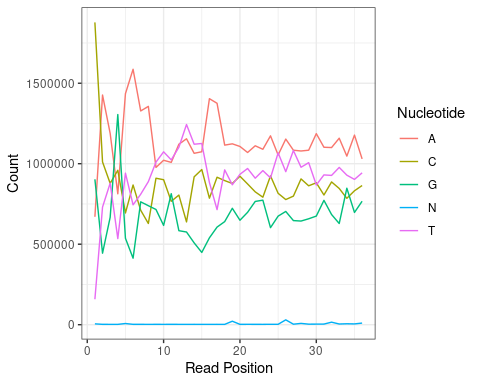
\includegraphics{hw4_files/figure-latex/position plot-1.pdf}

Early on in the reads there appear to be a large number of cytosines and
not many thymines. However, as the read position increases the
proportions seem to stabilize and there are generally more adenosines
and thymines, as one might expect.

\hypertarget{quality-score-boxplot}{%
\subsubsection{Quality score boxplot}\label{quality-score-boxplot}}

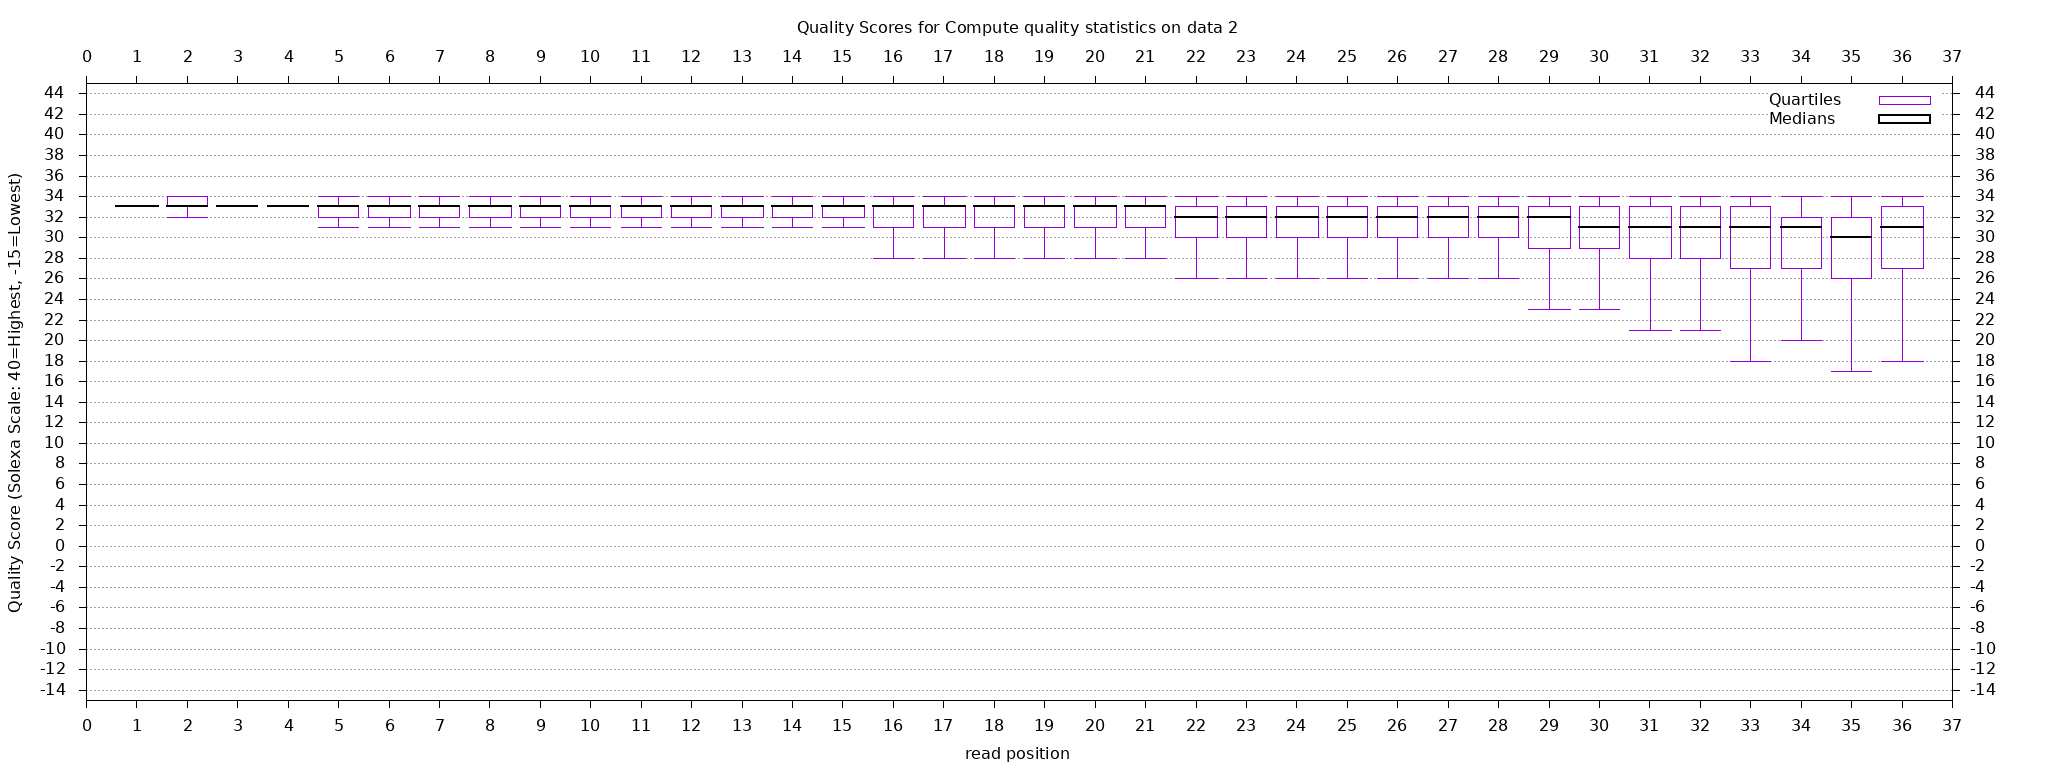
\includegraphics{./quality_score_boxplot.png}

As the read length increases, the quality tends to deteriorate. Based on
visual inspection it seems that the drop in overall quality occurs
around position 29.

\hypertarget{rna-seq-mapping-using-bowtie2}{%
\section{2. RNA-seq Mapping using
Bowtie2}\label{rna-seq-mapping-using-bowtie2}}

\end{document}
